\chapter{随机盲法试验的设计}
\chapterauthors{Steven R. Cummings、Deborah G. Grady、Alison J. Huang}
\begingroup\setlength{\tabcolsep}{4pt}
\sourcepage{332}
在\term{临床试验}中，研究者实施一项干预，并观察它对一个或多个结局的作用。如果试验采用随机化和盲法，其相对于观察性研究的主要优势，就是能够证明因果关系。随机分配干预可尽量减少混杂变量的影响；盲法则可尽量减少这样的可能性：干预的表面效果其实来自安慰剂效应、其他共同干预使用上的差异，或者结局报告与确定过程中的偏倚。

本章重点讨论随机盲法试验的设计，包括选择干预与对照条件，界定并测量结局和不良事件，选择参与者，以及确定随机化与盲法的方法。我们还讨论实施临床试验、分析结果的有关问题，以及预试验的价值。下一章将讨论其他试验设计。

\section{选择干预与对照条件}
“经典”的随机试验将参与者随机分配到待检验的干预，或某种对照；对照可以是不含活性成分的安慰剂，也可以是另一种治疗。最理想的是对分组设盲，使研究者、参与者及工作人员都不知道某位参与者被分配到干预组还是比较组。研究者给予活性干预及对照干预，随时间随访参与者，再比较两组结局（图11.1）。这种设计的名称有时加上“平行组”，表示干预组和对照组同时入组、同时随访。
% Figure 11.1 redrawn from PDF page 333. Figures 11.2 and 11.3 retain
% the original anatomical illustrations (PDF pages 362--363); only labels
% are covered by Chinese TeX text, leaving patient figures and colors intact.
\providecommand{\chElevenTrial}{\begin{tikzpicture}[font=\footnotesize,>=Stealth]
\draw[dashed,dcrred] (0,0) ellipse (2.6 and 2.8);\node[text=dcrred]at(0,3.1){可接触人群};
\node[align=center]at(0,2.1){符合选择标准的参与者};
\node[draw=dcrred,text width=36mm,minimum height=31mm,align=center,text=dcrpurple](b)at(0,0){测量基线变量\\[10pt]保存标本（可选）};
\node[circle,draw,minimum size=10mm](r)at(3.6,0){R};\draw[->](b)--(r);
\node[draw=dcrteal,text width=47mm,align=left](a)at(7.8,1.6){\textcolor{dcrblue}{实施设盲干预}\\测量依从\\\textcolor{dcrgold}{结局发生时测量}};
\node[draw=dcrteal,text width=47mm,align=left](c)at(7.8,-1.6){\textcolor{dcrblue}{实施设盲对照}\\测量依从\\\textcolor{dcrgold}{结局发生时测量}};
\draw[->,dcrteal](r)to[bend left=25](a);\draw[->,dcrteal](r)to[bend right=25](c);
\node[draw=dcrgold,text=dcrgold,align=center](e)at(11.5,0){也可在\\随访结束时\\测量结局};
\draw[->,dcrteal](a)--(e);\draw[->,dcrteal](c)--(e);
\foreach \yy in {1.6,-1.6}{\draw[->,dcrteal](7,\yy-.6)to[bend left=30](7.4,\yy-1.1);\draw[->,dcrteal](8.4,\yy-.6)to[bend left=30](8.8,\yy-1.1);\node[text=dcrteal]at(7.9,\yy-1.35){失访};}
\end{tikzpicture}}
\providecommand{\chElevenHip}{\begin{tikzpicture}[x=.018cm,y=-.018cm]
\node[anchor=north west,inner sep=0]at(0,0){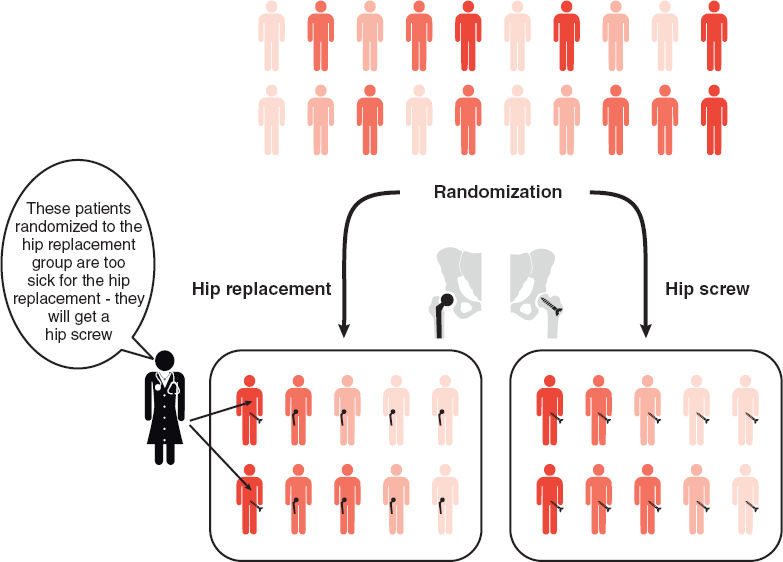
\includegraphics[width=14.094cm]{assets/ch11_figure02_original.png}};
\fill[white](403,174)rectangle(595,208);\node[font=\small]at(500,191){随机分组};
\fill[white](186,271)rectangle(334,305);\node[font=\small]at(260,289){髋关节置换};
\fill[white](653,271)rectangle(778,305);\node[font=\small]at(715,289){髋螺钉固定};
\fill[white](78,264)ellipse(73 and 100);
\node[text width=1.8cm,align=center,font=\scriptsize,fill=white]at(80,273){这些患者虽随机分入置换组，但病情太重，不适合置换，将改用螺钉固定。};
\end{tikzpicture}}
\providecommand{\chElevenAnalysis}{\begin{tikzpicture}[x=.018cm,y=-.018cm]
\node[anchor=north west,inner sep=0]at(0,0){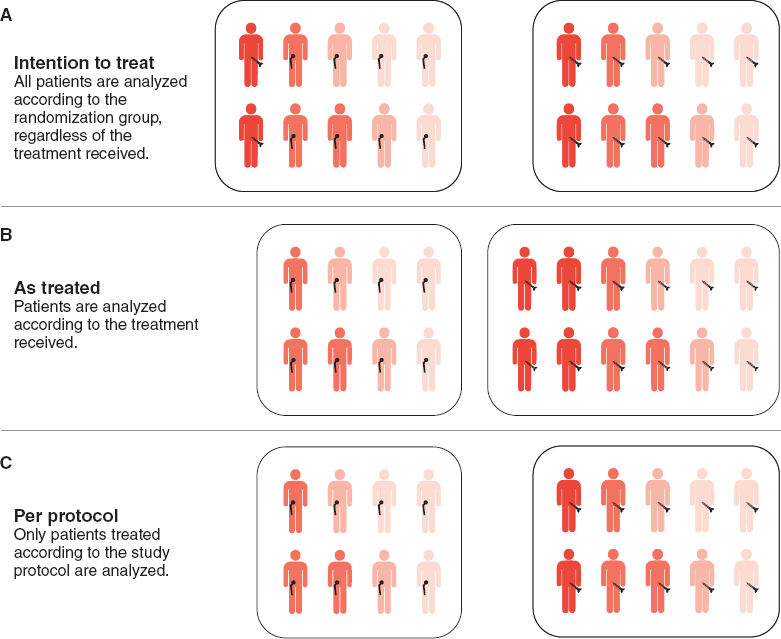
\includegraphics[width=14.058cm]{assets/ch11_figure03_original.png}};
\fill[white](5,35)rectangle(210,181);\node[anchor=west,text width=3.3cm,align=left,font=\small]at(14,103){\textbf{意向治疗分析}\\全部患者按随机分组分析，不管实际治疗。};
\fill[white](5,266)rectangle(210,390);\node[anchor=west,text width=3.3cm,align=left,font=\small]at(14,326){\textbf{按实际治疗分析}\\按实际接受的治疗分析。};
\fill[white](5,486)rectangle(210,609);\node[anchor=west,text width=3.3cm,align=left,font=\small]at(14,547){\textbf{符合方案分析}\\仅分析按研究方案治疗的患者。};
\end{tikzpicture}}

\sourcepage{333}
\begin{figure}[htbp]\centering\chElevenTrial
\caption*{\textbf{图11.1\quad 随机盲法试验。}从适合且能够安全接受干预的可接触人群中选择参与者样本；测量基线预测变量，以及适当情况下的结局变量基线水平；考虑额外测量并保存标本，以备后续分析；随机分配（以R表示）设盲的干预与对照条件（如安慰剂）；随访参与者，尽量减少失访，评估对干预和对照的依从性；在结局发生时或随访结束时测量结局变量。}
\end{figure}

\subsection{干预的选择}
选择干预是设计临床试验时至关重要的第一步。药物、行为干预项目和手术等各种干预，都需要考虑相似的问题，包括实施方式、剂量或强度、实施频次及持续时间。\sourcepage{334}选择时必须平衡几个目标：疗效与安全性、参与者的可接受性，以及实施的便利程度。

对于治疗严重疾病，或降低较高残疾、死亡风险的干预，\term{疗效}（efficacy），即治疗所关注疾病的有效程度，是设计时的首要考虑。在这些情况下，最好选择能够耐受的最高治疗剂量、频次和持续时间。对于后果较轻的疾病，尤其是对健康人实施预防性干预时，研究者必须更加重视安全性：即使有效，干预也只能预防或改善部分人的疾病，而每一位接受者都面临不良作用的风险。

有时，研究者可能决定将一种以上剂量或持续时间的干预与对照组比较。这可能是合理选择，但需要规模更大的试验。另一些情况下，最好允许滴定活性药物的剂量或行为治疗的强度，以获得最佳疗效。为维持盲法，对照组参与者的安慰剂“剂量”也应作相应改变。

检验单一干预的试验，比检验联合干预的试验容易规划和实施得多。运动联合饮食等组合最重要的缺点，是结果无法对其中任何单一成分得出明确结论。例如，女性健康倡议比较绝经后雌激素联合孕激素治疗与安慰剂，发现乳腺癌等多个结局的风险增加；但无法确定作用来自雌激素还是孕激素（1）。

研究者应考虑参与者愿意接受干预的程度、干预能否设盲，以及它在临床实践中的适用性。干预负担较小时，人们更愿意入组，也更可能依从。由多个难以标准化的成分构成的复杂干预，例如改变行为的多方面咨询，\sourcepage{335}可能难以复制、耗时或昂贵，因此难以融入一般实践。即使试验证明有效，这种干预也较难产生公共卫生影响。

\subsection{对照的选择}
最好的对照组也以一种能够设盲的方式接受“治疗”。对于药物，通常需要与试验药无法区分的安慰剂或另一种药物。这样可以抵消活性干预通过暗示或期待产生的\term{安慰剂效应}（placebo effect），使组间结局差异可以归于干预的特异作用。但教育、行为训练或医疗操作等干预，可能很难甚至无法构造盲法对照。

有些试验可以要求参与者在试验期间避免其他可能影响结局的治疗，例如骨质疏松新疗法研究中，不应服用其他治疗该病的药物。但往往不能停用这些治疗：一项在已有冠心病（CHD）患者中降低心肌梗死风险的试验，不能禁止或劝阻他们使用有临床指征的他汀等药物。一个解决方法是给全部参与者标准或通常照护，在此基础上，干预组加试验治疗，对照组加安慰剂。这回答了最相关的临床问题——新干预加在标准照护上是否改善结局——但会降低总体事件发生率，从而增加所需样本量。

\subsection{共同干预}
\term{共同干预}（cointerventions）是研究干预之外，能够改变所关注结局风险的治疗或行为。如果它在某组比另一组更常出现，问题尤其突出。例如，一项以力量训练改善帕金森病患者运动功能的试验中，对照组可能因为没有接受干预而增加步行，作为补偿。\sourcepage{336}如果运动等有效共同干预在两组使用不同，结果就会产生偏倚。

盲法可以尽量减少组间共同干预差异，详见后文。如果不能设盲，方案必须安排收集有关资料，例如定期客观测量运动量，以便统计调整共同干预使用上的差异。不过，共同干预可能难以测量；调整这种随机化后出现的差异，也违背本章后述的意向治疗原则，因此应把它视为次要或解释性分析。

\section{选择结局测量}
具体结局的选择和定义，会影响许多其他设计要素，以及试验成本和可行性。试验常纳入多个终点，使结果更丰富，并提供次要分析的可能性。但应始终指定一个\term{主要结局}（primary outcome），反映主要研究问题，指导样本量计算，并确定实施工作的优先次序。只有试验规模和持续时间能够提供足够统计效能，产生有意义的结果时，才应考虑次要终点。

卒中、骨折等临床结局风险的变化，或参与者健康、功能和生活质量的变化，最能说明干预的价值。不过，新发痴呆等许多临床结局并不常见，寻找有效治疗的试验因而必须规模大、时间长、成本高。如第6章所述，以标准工具测量的认知功能变化等连续结局，所需参与者少于二分结局。

\term{生物标志物}（biomarkers）是与临床结局相关的中间测量，通常在生物样本中测得。\sourcepage{337}例如，原先升高的白细胞计数下降，与肺炎成功治疗相关。但只有在既往同类治疗试验中，治疗引起的标志物变化能够一致预测临床结局的作用时，才能把它视为临床结局的\term{替代标志}（surrogate markers）（2）。例如，治疗相关的股骨颈骨密度变化，可以预测治疗降低骨折风险的程度：骨密度是骨强度的主要决定因素，也能预测骨折风险；既往试验的荟萃分析显示，股骨颈骨密度改善可预测髋部及非脊柱骨折减少（3）。很少有中间标志满足这些条件。即使能够预测临床结局，用作试验终点仍可能误导（2、4、5）。例如，较高的高密度脂蛋白（high-density lipoprotein，HDL）胆固醇和较低的LDL胆固醇，预测心血管病及死亡风险较低；但一项试验发现，torcetrapib虽对两者有非常有利的作用，却增加了全因死亡和心血管事件（6）。

\subsection{结局变量的数量}
采用多个结局变量，测量所关注现象的不同方面，往往是有益的。但次要结局过多，会使实施更复杂、成本更高。例如，在将COVID-19住院成人随机分到羟氯喹或安慰剂的试验中，主要结局是随机后14天的临床状态。这既便于确定样本量和研究时长，也避免了多重假设检验的解释问题。研究者还测量了恢复时间、不良事件等12项次要结局。主要结局及全部次要结局均未见益处，使他们可以更明确地得出治疗无效的结论（7）。

\sourcepage{338}
\subsection{复合结局}
有些试验采用\term{复合结局}（composite outcomes），将心肌梗死、冠脉血运重建和卒中等相关事件组合。如果各项都有临床意义，并受到干预的相似影响，这样做可能合理；由于事件更多，复合结局的效能高于单一结局。但组合生物机制或发生频率不同的事件，可能产生误导。如果冠脉血运重建远比其他成分常见，它就会主导复合结局，表面上降低“心血管事件”的干预，实际可能只减少血运重建。此外，治疗对冠脉血运重建和出血性卒中的生物作用可能不同，因此“心血管事件”减少，并不意味着对两者都有益。

\subsection{不良事件}
研究者还应确定干预或试验其他环节可能引起的\term{不良事件}（adverse events），例如用于评估动脉粥样硬化进展的冠状动脉造影所引起的事件。多数临床试验的重要目标，是判断有利作用是否超过不利作用，即使健康教育项目或癌症筛查等看似无害的干预，也不例外。不良事件可从上呼吸道感染等轻微症状，到结核再激活等严重乃至致死并发症。由于发现肾衰竭等罕见事件需要大样本，多数试验没有足够效能发现其风险增加。这类事件往往要等干预广泛用于临床后，才可能通过大型医疗数据库分析或病例报告发现，也可能始终未被发现。

在新干预测试的早期，潜在不良事件尚不明确，应使用开放式问题，询问是否发生任何不良事件。\sourcepage{339}还应根据既往研究或临床经验，对预计可能出现的重要事件设计专门问题。分析时应对事件分类。MedDRA（\url{www.ich.org/products/meddra.html}）和SNOMED（\url{https://www.nlm.nih.gov/research/umls/}）等标准词典，可按症状、诊断和器官系统等多种方式归类。不良事件也常按与干预相关的可能性及严重度分类。\term{严重不良事件}（serious adverse events）指致死或危及生命、需要或延长住院或医疗处理、导致残疾、永久损害或出生缺陷的事件（\url{www.fda.gov/Safety/MedWatch/HowToReport/ucm053087.htm}）。癌症等特定领域已有分类方法（\url{http://ctep.cancer.gov/protocolDevelopment/electronic_applications/ctc.htm}）。可能与干预相关，或出乎预期的严重事件，应及时向伦理审查委员会（IRB）和申办方报告。若试验资料将用于申请新药监管批准，设计必须满足不良事件报告方面的监管要求（\url{http://www.fda.gov/Drugs/InformationOnDrugs/ucm135151.htm}）。

\section{选择参与者}
第3章讨论了如何通过选择标准，界定适合研究问题的目标人群，如何设计有效率且科学的选择方法，以及如何招募参与者。这里讨论对临床试验尤其重要的问题。
\subsection{临床试验的选择标准}
试验必须招入并随访足够多、主要结局风险足够高的参与者，才有足够效能发现重要的干预作用（第5章）。\sourcepage{340}选择标准应平衡几个需要：纳入最可能获益者，招到预定人数，并尽量提高结果的可推广性。例如，若关注新发乳腺癌等少见事件，通常必须招募高风险者，才能把样本量和随访时间降到可行的程度。但将纳入标准限于高风险女性，会限制结果的可推广性，也更难招够人数。

规划样本量时，必须估计这些潜在参与者在未接受干预时的主要结局风险，或终点的变化速率。可以使用生命统计或纵向观察性研究，例如从登记资料估计胰腺癌预期死亡率。不过，研究者应记住，符合资格且同意参加试验的志愿者，往往比一般同病患者更健康；因此，试验事件率常低于目标人群，终点变化速率也可能不同。更好的估计来源，可能是纳入标准与计划试验相似的研究中的未治疗组。

目标人群的概率样本对观察性研究有优势，但在随机试验中通常既不可行，也没有必要。纳入特征多样的参与者，会增强结果广泛适用的信心，前提是女性、少数族裔等重要群体人数足够，以判断作用是否一致。不过，除非不同人群存在影响干预作用的生物或遗传差异，便利样本（如响应广告的冠心病女性）的试验结果，一般会与合格人群概率样本（全部冠心病女性）的结果相似。有时，干预作用确实取决于年龄或性别等协变量，这称为效应修饰（第10章）。

\sourcepage{341}按至少80岁等可能影响干预作用或结果推广的特征进行分层抽样，可以保证具有该特征者达到预定人数，达到目标后即可停止该层招募。但如果试验没有足够效能检验该亚组与其他人之间的作用差异，这种策略的价值可能有限。排除标准应尽量简约：不必要的排除会增加招够人数的难度，降低可推广性，并增加招募的复杂性和成本。不过，仍有数种理由可将某人排除在临床试验之外（表11.1）。

\begin{longtable}{L{70mm}L{79mm}}
\caption*{\textbf{表11.1\quad 临床试验排除参与者的理由}}\\\toprule
理由&低剂量甲氨蝶呤（MTX）预防动脉粥样硬化事件的例子（8）\\\midrule\endfirsthead
\toprule 理由&例子\\\midrule\endhead
1. 研究治疗可能有害：分至活性组有不可接受风险&酗酒史、不愿限制每周少于4杯（MTX与酒精有不良相互作用）\\
分至对照组有不可接受风险&需服改变叶酸代谢的药\\
2. 活性治疗可能无效：结局风险低&CHD风险极低的年轻成人\\
疾病类型不太可能响应&距既往心肌梗死或操作不足60天，再发事件较可能\\
服用可能与干预不良相互作用的治疗&需糖皮质激素或其他免疫抑制治疗\\
3. 不太可能依从&初始MTX导入期依从差\\
4. 不太可能完成随访&试验结束前计划搬迁，无法测末次结局；预期寿命不足3年，结局随访时间不够\\
5. 实际参与困难&认知受损，不能准确回答\\\bottomrule
\end{longtable}
\sourcepage{342}
如果活性或对照干预对某位潜在参与者不安全，就应排除。例如，主要经肾排泄的药物试验通常排除晚期肾病患者；严重抑郁者不应进入新抗抑郁药的安慰剂对照试验。对活性干预不太可能有效者、不太可能依从者，以及不太可能完成随访者，也应排除。有时，认知状态受损或语言障碍使其难以遵循指令，也构成实际理由。但糖尿病或年龄上限等影响许多人的标准，可能大幅影响招募可行性、费用及结果推广，必须仔细权衡。

\subsection{确定足够样本量并据此规划招募}
如果试验没有规划足够人数来检出重要作用，可能产生误导性结论，因此可以认为既浪费资源，也不合伦理。样本量估计是早期规划最重要的工作之一。\sourcepage{343}估计时应认识到，健康志愿者偏倚通常使试验事件率低于预期。此外，参与者必须愿意随机接受安慰剂或“实验性”治疗，并依从干预，招募往往比观察性研究更困难。因此，应计划从较大的可接触合格人群招募，并准备足够资源，在障碍一如常见地超过预期时，仍能达到预定人数。

\section{基线变量测量}
\subsection{描述参与者}
除充分的联系方式外，研究者还应收集结局危险因素，以及可能影响干预疗效和风险的其他特征。这些测量可以检查随机组的基线可比性，并评估结果的可推广性。目的是确认基线差异没有超过偶然所能解释的程度，否则可能提示随机实施中的技术错误或偏倚。小试验容易仅因偶然而出现较大不均，测量重要结局预测因素，有助于随后统计调整。它也能帮助研究者考察不同亚组的干预作用是否不同，即效应修饰（第10章）。

\subsection{测量结局变量的基线值}
如果结局定义为某变量的变化，研究开始时必须用与结束时相同的方法测量该变量。对于疼痛严重度评分等连续结局，几乎总以研究期间的变化作为最佳指标；这种方法通常比仅比较终点值有更高效能。\sourcepage{344}对于肺癌发生等二分结局，则常有必要通过病史、体检和诊断检查，证明试验开始时尚无该结局。

\subsection{额外测量}
尽管基线测量有许多用途，随机试验的设计本身并不要求测量任何基线变量，因为随机化已尽量减少研究开始时各因素造成的混杂。增加测量可回答更多问题，却增加复杂性和费用。预算有限时，把时间与资金用于保证样本充足、随机化和盲法成功、干预依从性良好及随访完整等重要方面，可能更值得。

\subsection{保存标本}
如果参与者在基线提供血液、组织或其他生物标本，保存这些样本，可供以后测量治疗引起的变化、预测结局的标志物，以及基因型等可能识别治疗反应良好或不佳者的因素。保存标本也可成为研究与主要结局无关问题的丰富资源。

\section{随机化与盲法}
任何试验的一个关键步骤，都是把参与者随机分到两组或更多组。最简单的设计是一组接受活性干预，另一组接受无活性安慰剂或其他干预。除偶然变异外，随机化使可能混杂所见关联的基线特征——包括未知或未测量的特征——在各随机组中均等分布。盲法则有助于减少差异性的安慰剂效应，\sourcepage{345}维持试验期间的组间可比性，并确保结局确定没有偏倚。

\subsection{随机化}
每位参与者都必须在随机化前完成筛查、确认符合资格，并同意入组，然后才随机分配。简单试验使用计算机算法生成治疗分配，可在研究现场完成，也可由发放活性或对照药物的研究药房完成。多数多中心试验设中央随机机构，当现场有合格者准备随机时与其联系。计算机不可行时，简单试验偶尔可将分配放在不透明信封内，于入组时打开。随机过程必须防止操纵，因为研究者可能受到影响分配的压力，例如希望某个看起来特别适合活性治疗的人，在安慰剂试验中进入活性组。

\subsection{特殊随机方法}
通常将参与者等比例随机分到各干预组。在小型至中型试验中，采用特殊方法来平衡各组人数，即\term{区组随机化}（blocked randomization），以及平衡结局基线预测因素的分布，即\term{分层区组随机化}（stratified blocked randomization），可略微提高效能。

盲法试验使用预定大小的区组，使各组人数均等。例如区组大小为6，在每六人中照常随机，直到其中一组达到三人，再把其余人分到另一组，完成该区组。因此，30人的试验会恰好每组15人；33人时，不均最多为18:15。\sourcepage{346}固定区组大小较不适合非盲试验，因为每个区组末尾的分配可被预见和操纵。可按研究者不知道的安排，随机改变区组大小，例如在4～8人之间变化，以减少此问题。

分层区组随机化使重要结局预测因素的组间分布，比仅靠偶然更均匀。例如，肥胖是运动预防糖尿病试验中很强的预测因素，最好确保两组肥胖者人数相近；可在肥胖与非肥胖两个层内分别区组随机。它减少重要基线因素偶然不均带来的结局变异，可略增小试验效能。大型试验随机分配已使分布近乎均等，受益很少。其重要限制是只能平衡少数、通常两三个基线变量。\term{适应性随机化}（adaptive randomization）可用“有偏硬币”改变每位新参与者的分配概率，解决此限制：按任意多个基线预后变量计算的高风险者，会略更可能分到当时平均风险较低的组。它需要交互式计算系统，在每次随机化后重新计算概率。

通常最好使各组人数相等，因为在给定总样本量下效能最高。不过，即使2:1的不均，效能损失也有限（9）；有时可以不等分配治疗与对照（10）：\sourcepage{347}
\begin{itemize}
\item 增加活性组比例，可以吸引希望有更大机会接受活性治疗的潜在参与者。
\item 增加活性组比例，可以扩大该组研究中介变量的样本。例如PRIDE试验将超重或肥胖参与者的三分之二分到强化行为减重组（11）。
\item 干预非常昂贵时，减少接受者比例，可使试验费用可以负担，如女性健康倡议的低脂饮食试验（12）。
\item 若一个对照组服务于多个活性干预组，增加对照比例可以提高其估计精度，从而提高每项比较的效能，如冠心病药物项目（13）。
\end{itemize}

匹配对随机化是另一种平衡基线混杂的方法：先按年龄、性别等重要特征配对，再随机使一人进入一个组。它增加招募复杂性，因为合格者必须等到找到合适匹配者才能随机；大型试验随机化已能平衡，也不需要匹配。不过，如果情形允许在同一人两个部位比较活性与对照，便有一种很有吸引力的变体。例如，部分亚洲人因遗传而容易酒后面部潮红。一项试验随机在受此困扰者的一侧面颊涂溴莫尼定（brimonidine，α肾上腺素能受体激动剂）凝胶，另一侧涂安慰剂（14）。比较同一人两颊变化，显示活性凝胶减少了饮酒后的红度。

\subsection{盲法}
如果知道干预分配可能影响结局评估，对评估设盲就很重要。\sourcepage{348}应尽可能使研究者、参与者、与参与者接触的工作人员、测量人员，以及确定和判定结局者均不知道分配。如果不能全部设盲，尤其应对参与者和作出结局判断的人员设盲。这可尽量减少差异性的安慰剂效应与共同干预，以及结局确定、判定的偏倚，自报症状等主观结局尤其如此。例如，新干预旨在减轻疲劳时，知道自己组别的人，可能因相信干预会改善精力而改变疲劳感受。对已报告结局的判定者也必须设盲：若结局为心肌梗死，可收集症状、心电图和心酶资料，再由不知分组的专家按明确标准判定。

加拿大合作多发性硬化试验说明了盲法对无偏结局判定的重要性（15）。患者被随机分到血浆置换联合或不联合环磷酰胺和泼尼松，或假血浆置换加安慰剂药物。结束时，先由不知分组的神经科医师用结构化检查评估严重度，再由未设盲医师评估。前者认为治疗无效，后者却认为有效。未设盲医师并非有意使结果偏倚，但人们有强烈愿望看到治疗后改善，尤其当治疗痛苦或可能有害时。盲法可以尽量减少这种判定偏倚。

死亡等“硬”结局，或血糖等自动测量，可能较不容易出现评估、报告偏倚。但\sourcepage{349}死因、疾病诊断、体格测量、问卷量表及自报状况等多数其他结局，都易受确定和判定偏倚影响。结束时让参与者和研究者猜分组，常是有益的做法；两组中猜自己被分到活性干预的比例应相近。如果不同，发表结果时应在讨论中评估破盲可能造成的偏倚。

\subsection{难以或无法设盲时}
盲法并非总能实现，例如把运动干预与仅收到宣传册的对照比较。外科干预也难设盲，因为给对照做假手术可能看似不合伦理。不过，手术等侵入性操作总有风险，向公众推荐前必须确定它确实有效。手术也可能影响参与者的共同干预使用及健康感受，因此未盲试验易受共同干预差异和结局报告偏倚影响。例如，接受冠脉成形、支架置入者可能预期胸痛改善；但将有症状冠心病患者随机到成形术或完全相同、仅不处理动脉病变的假操作，结果自报症状没有差异（16）。在此例中，获取这种常见治疗疗效的充分资料，比对照承担的风险更为重要。许多行为干预也有相似考虑，可用省去关键治疗成分、仅让参与者接受非指导性治疗的假干预。

如果无法对干预分配设盲，仍应确保结局判定者设盲，并主动限制共同干预。例如，在瑜伽缓解腰痛试验中，\sourcepage{350}可要求瑜伽组和对照组在试验结束前都不要开始新的腰痛治疗。收集疼痛严重度资料的工作人员也不应同时提供瑜伽训练，因为他们可能记得谁属于活性组。

即使干预性质使参与者无法设盲，也可促进两组间的临床均势，减少对疗效的期待差异，从而减少差异性安慰剂效应、共同干预和结局报告偏倚。例如，腰痛瑜伽试验可给对照一种需要相似时间和注意投入的身体活动项目，避免两组参与程度不同。这种对照也可能提供其他合理的健康益处，帮助招募和保留那些希望时间投入有所回报的人。

\section{预试验}
有时，先开展小型研究，收集规划较大临床试验所需的信息很有价值，例如确定最佳招募方法及临床访视所需时间。\term{预试验}（pilot studies）不适合估计拟用干预的疗效，因为样本小，估计容易不精确。附录11A介绍其用途。

\section{嵌入医疗服务的试验}
多数试验在临床环境开展，安排面对面访视、测量和资料收集。但其他环境也能支持随机试验。例如，现在可以借助电子病历系统，在提供医疗服务的同时实施干预、收集资料。这种“嵌入式”试验最常研究临床流程的质量改进。\sourcepage{351}其中有些是经典随机盲法试验，另一些则采用前后或中断时间序列设计（第12章）。

\section{为新干预监管审批开展试验}
许多试验在美国食品药品监督管理局（FDA）或其他监管机构批准上市前，检验新治疗的有效性和安全性；也有试验考察已获某适应证批准的药物，能否治疗或预防其他疾病。这些试验的设计、实施与其他试验相同，但必须考虑监管要求。

FDA发布有关实施指南。以获得新药或器械批准为目标的研究者和人员，应接受\term{药物临床试验质量管理规范}（Good Clinical Practice）等一般指南的专门培训。FDA也对某些结局给出具体指导，例如本版撰写时，申请绝经潮热疗法批准的研究，必须纳入每天至少7次或每周50次潮热者。FDA定期更新指南，其他国际监管机构也提供类似指南。

新治疗监管试验按“期”描述，表示有序推进的测试过程。首先在动物、人细胞培养或组织中开展临床前研究；I期在少量志愿者中以未盲、无对照治疗初步检验安全；II期用小型随机或时间序列试验，测试多个剂量对不良作用、生物标志或临床结局的影响；III期则用足够大的随机试验，检验治疗是否以可接受的安全性改善血压等目标状况，或降低卒中等疾病风险（表11.2）。FDA通常规定新药上市审批所需III期试验的终点。\sourcepage{352}IV期是在批准后开展的大型研究，可能随机，但更常为观察性研究，用来评估大人群中的严重副作用发生率，或检验其他用途。

\begin{table}[htbp]\centering\small
\caption*{\textbf{表11.2\quad 新疗法试验阶段}}
\begin{tabularx}{\textwidth}{L{22mm}Y}\toprule
临床前&细胞培养、组织和动物研究\\
I期&在少量志愿者中开展未设盲、无对照研究，检验安全性\\
II期&规模较小的随机试验或时间序列试验，检验耐受性，以及不同干预强度或剂量对生物标志物或临床结局的作用\\
III期&规模较大的随机盲法试验，对治疗影响临床结局和不良事件的作用作出明确检验\\
IV期&治疗经FDA批准后开展的大型试验或观察性研究，评估不常见严重副作用的发生率，并提出其他可能的治疗用途\\\bottomrule
\end{tabularx}
\par\smallskip{\footnotesize FDA：美国食品药品监督管理局。}
\end{table}

\section{实施临床试验}
\subsection{随访与依从方案}
为实现确定干预作用的目标，参与者必须依从方案，并提供随访资料。因此，规划试验时必须认真考虑如何尽可能提高依从性和随访完成率，避免最终结果效能不足或产生偏倚（表11.3）。

\begin{longtable}{L{49mm}L{100mm}}
\caption*{\textbf{表11.3\quad 尽量完成随访并提高方案依从性}}\\\toprule
原则&例子\\\midrule\endfirsthead
\toprule 原则&例子\\\midrule\endhead
选择可能依从干预与方案的参与者&要求随机化前完成至少两次访视；排除随机化前导入期不依从者；排除可能搬迁或不配合者\\
使干预简单&可能时，采用每日一次、每次一片的用药方式\\
使研究访视方便、愉快&与参与者建立良好的人际关系；通过电话、电子邮件或远程电子设备收集资料；考虑在家中测量并提供治疗，替代到诊所访视；提供晚间或周末门诊；配备充足、组织有序的工作人员，避免等待；报销交通与停车费用\\
使研究测量无痛、有趣&优先采用非侵入性检验；向参与者提供他们感兴趣的检验结果，适当时提供咨询或转诊\\
鼓励参与者继续参加试验&绝不因违反方案、发生不良事件或停止干预而终止随访；发送通讯简报和电子邮件；强调依从与随访的重要性；向参与者寄送生日和节日贺卡\\
寻找失访参与者&询问参与者的密切联系人；使用人员追踪服务\\\bottomrule
\end{longtable}
\sourcepage{353}
参与者未接受干预的程度越大，观察到的活性作用就越弱。应尽可能把干预设计得易用、耐受良好；每日一次或更少服用的药物最容易记住，因而更可取。需要数小时练习的行为干预，依从性可能较低。方案应安排提高依从性的措施，例如要求在每天早晨固定环节服药，\sourcepage{354}提供标有星期几的药盒，或发送手机提醒。对于行为干预，则可强化或奖励参加训练。

还须考虑如何测量干预依从性，例如自报、药片计数、记录开盒时间的传感药盒、干预练习日记或日志，以及与干预使用相关的血清或尿代谢物水平。这可识别未依从者，以便采取改进措施，并帮助正确解释结果。

在取得同意前说明研究要求，安排便利时间并配备足够人员以避免等待，每次访视前一天电话或邮件提醒，以及报销交通、停车等自付费用，都能提高访视和测量的依从性。下节所述的居家评估可消除到临床机构的障碍和不便（17）。让参与者感到自己受到感谢很重要；他们常说，与研究人员的个人关系，是继续访视及依从治疗的最重要理由之一。

未能随访并测量所关注结局，会造成偏倚，削弱结果可信度，并降低统计效能。例如，一项鼻喷降钙素预防骨质疏松性骨折的试验报告风险降低36\%（18），但约60\%随机参与者失访，不知道是否骨折。由于总骨折数少，即使失访者中仅有少数骨折，也可能改变结论；这种不确定性削弱了结果的可信度（19）。

即使参与者违反方案或停止干预，也应继续随访，使其结局可用于\sourcepage{355}意向治疗分析，详见后文。许多试验因参与另一研究、漏访或停干预而终止随访，这可能使结果偏倚或无法解释。例如，某药副作用常使人停药，若副作用与主结局或严重不良事件有关，不随访停药者就可能造成偏倚。

研究开始时应告知随访的重要性，并记录一两名始终知道参与者居所的亲友姓名及联系方式。这既有助于确定生死状态，也使研究者可能通过电话或邮件，从拒绝最终现场访视者取得代理结局指标。

随机化前的筛查访视和导入期，是两项可能改善依从性、随访完成率的试验特有安排。要求先参加一两次筛查，可排除发现自己无法完成访视的人。难点在于门槛要足以排除日后不依从者，又不能高到把本可良好依从者也排除。

\term{导入期}（run-in period）可能提高依从干预和随访者的比例。在基线期间，全部参与者服安慰剂，经过预定时间、通常数周后，只有依从者，例如服用了至少80\%安慰剂者，才随机分组。这样在随机前排除不依从者，可提高效能，更好估计干预完整作用。但它会延迟入组，排除比例通常较小，\sourcepage{356}而活性组可能察觉随机后药物的变化，导致破盲。安慰剂导入是否比要求完成一次以上筛查更能提高依从性，也不明确。若没有具体理由怀疑依从性会差，就没有必要安排导入期。

另一种方法是在导入期给予活性药。除提高入组者依从性外，还可选出耐受并对干预响应的人；无不良事件，或与结局相关的生物标志物出现所需变化，都可作随机资格。例如，持续硝酸甘油治疗潮热的安慰剂对照试验，采用活性导入，排除因头痛停药的女性（20）。它提高活性组耐受、可能依从者比例，从而尽可能提高效能，但不能推广至被排除者。

活性导入还可能低估不良事件率。例如，卡维地洛对1094名充血性心衰患者死亡作用的试验中，两周活性导入期间17人心衰加重、7人死亡（21）。这些人没有随机入组，其药物不良事件也没有作为结局计入。

\subsection{传统临床机构外的试验}
一些有时称为“虚拟”“远程”或“分散”的试验，至少部分在临床机构之外进行，例如在线招募并在家完成试验（17）。在线减重等行为干预常如此，但药物和补充剂试验也可减少甚至不使用现场访视：在线知情同意和资格评估，把治疗送到家中实施，\sourcepage{357}由采血员上门或在当地实验室取得标本，通过自报及病历评估结局。不设实体临床机构，可不受地域限制、在任何时段招募，可能触及更多人。由于没有现场人员帮助，方案必须简单，招募和随访系统也必须直观，使参与者少需协助甚至无需协助即可完成。

\subsection{监测试验}
即使研究者起初认为试验程序不会造成过度风险，也未剥夺已知益处，这种判断仍可能在试验中改变。其他研究的新资料可能改变预期益害比，甚至回答本试验的问题。虽然同一问题有多项研究通常有价值，但如果期间出现明确的获益或伤害资料，继续可能不合伦理。

试验内部早期趋势，也可能提示作用比预期更有益或更有害。招募、依从或结局评估困难，还可能降低获得明确答案的机会。研究者必须确保参与者既不被不当地暴露于有害干预，也不被剥夺有效干预，更不能在问题不太可能获得回答时继续参加。试验期间须监测这三方面，决定是否应提前停止。
\begin{itemize}
\item \textbf{因伤害停止。}监测试验最迫切的理由，是确认干预没有出现意外伤害。如果判断伤害超过益处，就应停止。
\item \textbf{因获益停止。}若干预疗效高于设计时估计，可能较早就出现统计显著的益处。\sourcepage{358}一旦已明确证明获益，继续并延迟向安慰剂参与者及其他潜在获益者提供干预，可能不合伦理。
\item \textbf{因徒劳停止。}如果继续招募改变问题答案的概率极低，继续也可能不合伦理。例如计划5年的试验，在4年时两组事件率仍很接近，给定已有结果、在剩余时间拒绝零假设的\term{条件效能}（conditional power）就会很小，应考虑停止。有时因无法招募或保留足够人数，或无法维持足够治疗依从性，也会提前停止。
\end{itemize}
附录11B有实例。

多数临床试验都应有中期监测计划；NIH等资助机构可能明确要求。对于干预预计安全的小试验，研究者可以自行监测，也可指定一名独立数据与安全监察员。大型试验，或干预不良事件未知、可能危险的试验，通常由\term{数据与安全监察委员会}（Data and Safety Monitoring Board，DSMB）监测。成员包括相关疾病专家、生物统计学家、临床试验专家、伦理学者，有时还有患者代表。他们不参与试验本身，也不应因试验继续而有个人或财务利益。开始前应书面明确其指南和程序。

中期监测计划可以预定定期评估干预对主要结局及安全性的作用，以尽早发现获益、伤害或徒劳。统计方法必须补偿多次查看结果的影响。\sourcepage{359}反复分析相当于多重假设检验，会增加I类错误。例如，每次均用$\alpha=0.05$，试验期间分析四次、结束时再分析一次，I类错误概率会从5\%升至约14\%（22）。因此，中期方法通常降低每次检验的$\alpha$，使总体保持接近0.05。

停止试验必须慎重，平衡对参与者的伦理责任与科学知识的增进。应考察中期作用趋势在不同时点、不同亚组是否一致。有时修改比全停更好，例如延长随访，或停止结局不太可能发生的低风险亚组。任何提前停止都会失去获得更明确结果的机会，尤其是长期使用的不良事件；也可能削弱可信度，限制重要次要问题的回答能力（附录11B）。

贝叶斯试验的监测方法不同：不在指定时点检验统计学显著性，而随资料积累持续更新治疗可能的疗效（附录12A），因此没有基于$P$值的停止规则。

\subsection{结果分析：意向治疗分析、符合方案分析与按实际治疗分析}
临床试验主要假设的统计分析，比较分配到干预组与分配到对照组者的结局。这称为“一经随机，始终分析”或\term{意向治疗分析}（intention-to-treat analysis）：即使参与者从未接受所分配的干预或对照，也仍按随机组比较。只有不论是否依从都完成随访测量，才能按此原则分析。\sourcepage{360}因此，即使参与者提前停用干预或依从很差，也必须收集结局资料。

意向治疗分析保留随机化的主要好处：两比较组的潜在混杂变量分布相似。这有助于确保干预本身，而非任何已测或未测的基线差异，是组间结局差异的唯一因果解释（见第10章反事实框架）。种族／族裔和性别等变量，只有偶然分布不均时才会混杂干预与结局的因果关系；这种情况不常见，在大型试验中尤其如此。

在意向治疗分析中，发生\term{交叉}（cross over）的参与者——活性组未接受或不依从干预者，以及对照组最终接受活性干预者——仍按原随机分组，即原本打算给予的治疗分析。这样可能低估干预的完整作用，但能防止混杂。

相比之下，\term{符合方案分析}（per-protocol analysis）只纳入依从方案者。定义不尽相同，但常要求两组均依从分配的干预，完成规定比例的访视或测量，且无其他方案违反；未遵守者被排除。另一种\term{按实际治疗分析}（as-treated analysis），把接受干预或对照者按实际治疗归组，即使与随机分配相反；既未接受干预也未接受对照者被排除。这些分析看似合理，因为只有实际接受干预才可能受影响。但依从治疗及方案者，几乎总与未依从者在重要方面不同，\sourcepage{361}这些差异可混杂干预与结局的因果关系。

意向治疗把未接受指定干预者也纳入其作用估计，因此，大量停用或组间交叉会低估治疗作用的大小。这也是常同时采用意向治疗与符合方案分析的原因。如果两者疗效结果不同，应采用保留随机化价值的意向治疗估计。此外，与符合方案分析不同，意向治疗只能使作用估计向保守、即有利于零假设的方向偏移。不过，估计伤害时，按实际治疗或符合方案分析提供更谨慎的估计，因为干预只有在实际接受者中才可能造成伤害。

一项老年髋部骨折随机试验比较内固定（用螺钉把骨折复位固定）与人工髋关节置换（23）。置换组229人中，有5人最终改为螺钉，因为他们被认为病情太重，不能承受更长、风险更高的置换手术（图11.2）。
\sourcepage{362}
\begin{figure}[htbp]\centering\chElevenHip
\caption*{\textbf{图11.2\quad 比较髋关节置换与髋螺钉固定治疗髋部骨折的随机试验（23）。}患者并不总是接受其随机分组所规定的治疗。如果未按方案治疗者在某些方面与其他人不同，例如像图中一样病情更重（深红色），问题就尤其突出。为便于区分，图中将右髋画为关节置换，左髋画为螺钉固定。Martina Steurer绘；引自Newman TB、Kohn MA，\textit{Evidence-Based Diagnosis: An Introduction to Clinical Epidemiology}第2版（2020），经Cambridge University Press许可转载。}
\end{figure}
图11.3显示未接受所分配治疗者的三种分析办法。面板A的意向治疗分析仍按原组，保留随机化，但可能使结果趋向无组间差异。面板B按实际治疗分析，却对螺钉组尤其不公平，因为它现在包括一些原分到置换组的最高风险患者。\sourcepage{363}面板C的符合方案分析同样不公平：它从置换组排除了高风险者，却把螺钉组的高风险者保留下来。
\begin{figure}[htbp]\centering\chElevenAnalysis
\caption*{\textbf{图11.3\quad A—C，随机试验中未完全依从所分配治疗时的三种分析方法。}Martina Steurer绘；引自Newman TB、Kohn MA，\textit{Evidence-Based Diagnosis: An Introduction to Clinical Epidemiology}第2版（2020），经Cambridge University Press许可转载。}
\end{figure}
其他临床情况下，交叉可能双向发生，交叉者风险也可能较低而非较高。但原则相同：偏离所分配治疗者并非随机样本，\sourcepage{364}按实际治疗分析，或把他们排除，都很可能引起偏倚。

\subsection{亚组分析}
亚组分析在按性别等划分的参与者子集中，分别比较干预和对照。主要目的是寻找效应修饰，例如治疗作用是否因男女而异。由于易误用并导致错误结论，亚组分析评价不一；但谨慎使用可以提供有用信息，扩展试验推断。

为保留随机化价值，应按干预实施前的测量界定亚组。例如，地舒单抗使总体非椎体骨折风险降低20\%的试验，其预先计划的亚组分析发现，治疗在基线骨密度低的女性中有效，风险降低35\%，在较高者无效，效应修饰$P=0.02$（24）。按随机化后因素，例如治疗依从性，划分亚组则不保留随机化价值，常会误导。

即使按随机化前因素划分，也仍有问题。第一，亚组人数少于全试验；如果未显著可能仅因效能不足，不能声称药物在该组“无效”。第二，研究者常考察许多亚组，增加仅因偶然发现不同作用的可能性。应在试验前界定计划分析的亚组，并报告共分析了多少亚组（25）。若声称亚组反应不同，应有治疗效应按该特征划分后存在统计显著差异的依据；\sourcepage{365}还应在另一研究中确认，才把效应修饰视为成立。

\section{小结}
\begin{enumerate}
\item 设计和实施恰当的随机盲法试验，为循证医学与实践指南提供最明确的因果推断。
\item 干预及剂量的选择，需要平衡疗效与安全性。还应考虑临床实践相关性、能否设盲，以及是否联合多种药物。
\item 可能时，比较组应接受安慰剂或其他药物，使参与者、研究者及工作人员能够设盲。
\item 疼痛、生活质量、癌症发生及死亡等临床相关结局，最有意义。骨密度变化等中间结局，只有在治疗引起的标志变化能预测临床结局变化的程度上，才是有效的替代标志。
\item 测量多个结局有时有益，但是否合为复合结局，必须慎重考虑。应指定单一主要结局来检验主要假设。
\item 全部临床试验都应测量潜在不良作用，包括使用开放式测量，并设程序，及时向IRB及申办方报告严重不良事件。
\item 参与者应最可能获得益处、较少受到伤害，并依从治疗与随访。选择高风险者可减少样本量，但可能更难招募，也会降低可推广性。
\item 基线变量应描述参与者特征，并测量结局危险因素及基线值，以便日后考察特定亚组的干预作用；还应考虑保存生物标本。\sourcepage{366}
\item 随机化尽量减少基线混杂，分配过程必须防操纵。小试验可用分层区组随机化，减少主要预测因素的偶然不均。
\item 干预盲法有助于控制差异性的安慰剂效应、共同干预，以及结局确定与判定偏倚。
\item 预试验可检验可行性，估计时间和费用，但规模太小，不能精确估计干预作用。
\item 鼓励参与者完成随访并依从治疗至关重要；随访不全、依从不佳，会减弱或歪曲观察到的疗效与安全性差异。
\item 导入期可以排除不依从，或易出现早期治疗不良作用的潜在参与者。
\item DSMB应定期以未设盲分析监测治疗安全性与疗效。若不良作用或疗效有重要差异，或继续已不太可能显示差异，可提前停止。
\item 按原随机分配进行的意向治疗疗效分析，保留随机化价值；符合方案分析则是评估不良作用较谨慎的方法。
\item 亚组分析可揭示不同患者群的作用差异，但其效能较低，表面差异也可能仅因偶然，因此可能误导。
\end{enumerate}
\begin{references}
\item The Women’s Health Initiative Study Group. Design of the women’s health initiative clinical trial and observational study. Control Clin Trials. 1998;19:61-109.
\sourcepage{367}
\item Califf R. Biomarker definitions and their applications. Exp Biol Med. 2018;243:213-221.
\item Black DM, Bauer DC, Vittinghoff, E, et al. Treatment-related changes in bone mineral density as a surrogate biomarker for fracture risk reduction: meta-regression analyses of individual patient data from multiple randomised controlled trials. Lancet Diabetes Endocrinol. 2020;8(8):672-682.
\item Nissen SE, Wolski K. Rosiglitazone revisited: an updated meta-analysis of risk for myocardial infarction and cardiovascular mortality. Arch Intern Med. 2010;170(14):1191-1201.
\item The Action to Control Cardiovascular Risk in Diabetes Study Group. Effects of intensive glucose lowering in type 2 diabetes. N Engl J Med. 2008;358:2545-2559.
\item Barter PJ, Caulfield M, Eriksson M et al. Effects of torcetrapib in patients at high risk for coronary events. N Engl J Med. 2007;357:2109-2122.
\item Self WH, Semler MW, Leither LM, et al. Effect of hydroxychloroquine on clinical status at 14 days in hospitalized patients with COVID-19: a randomized clinical trial. JAMA. 2020;324:2165-2176.
\item Ridker PM, Everett BM, Pradhan A, et al. Low-dose methotrexate for the prevention of atherosclerotic events. N Engl J Med. 2019;380(8):752-762.
\item Friedman LM, Furberg C, DeMets DL. Fundamentals of Clinical Trials. 4th ed. Springer; 2010.
\item Avins AL. Can unequal be more fair? Ethics, subject allocation, and randomised clinical trials. J Med Ethics. 1998;24:401-408.
\item Subak LL, Wing R, West DS, et al. Weight loss to treat urinary incontinence in overweight and obese women. N Engl J Med. 2009;360(5):481-490.
\item Prentice RL, Caan B, Chlebowski RT, et al. Low-fat dietary pattern and risk of invasive breast cancer: the women’s health initiative randomized controlled dietary modification trial. JAMA. 2006;295:629-642.
\item CDP Research Group. The coronary drug project. Initial findings leading to modifications of its research protocol. JAMA. 1970;214:1303-1313.
\item Yu WY, Lu B, Tan D, et al. Effect of topical brimonidine on alcohol-induced flushing in Asian individuals: A randomized clinical trial. JAMA Dermatol. 2020;156(2):182-185.
\item Noseworthy JH, Ebers GC, Vandervoort MK, et al. The impact of blinding on the results of a randomized, placebo‐controlled multiple sclerosis clinical trial. Neurology. 1994;44(1):16.
\item Al-Lamee R, Thompson D, Dehbi HM, et al. Percutaneous coronary intervention in stable angina (ORBITA): a double-blind, randomised controlled trial. Lancet. 2018;391(10115):31-40.
\item Cummings SR. Clinical trials without clinical sites. JAMA Intern Med. 2021;181:680-684.
\item Chesnut CH 3rd, Silverman S, Andriano K, et al. A randomized trial of nasal spray salmon calcitonin in postmenopausal women with established osteoporosis: the prevent recurrence of osteoporotic fractures study. PROOF Study Group. Am J Med. 2000;109(4):267-276.
\item Cummings SR, Chapurlat RD. What PROOF proves about calcitonin and clinical trials. Am J Med. 2000;109(4):330-331.
\item Huang AJ, Cummings SR, Schembri M, et al. Continuous transdermal nitroglycerin therapy for menopausal hot flashes: a single-arm, dose-escalation trial. Menopause. 2016;23(3):330-334.
\item Pfeffer M, Stevenson L. Beta-adrenergic blockers and survival in heart failure. N Engl J Med. 1996;334:1396-1397.
\item Armitage P, McPherson C, Rowe B. Repeated significance tests on accumulating data. J R Stat Soc. 1969;132A:235-244.
\item Parker MJ, Pryor G, Gurusamy K. Hemiarthroplasty versus internal fixation for displaced intracapsular hip fractures: a long-term follow-up of a randomised trial. Injury. 2010;41(4):370-373.
\item McClung MR, Boonen S, Torring O, et al. Effect of denosumab treatment on the risk of fractures in subgroup of women with postmenopausal osteoporosis. J Bone Mineral Res. 2012;27:211-218.
\item Wang R, Lagakos SW, Ware JH, et al. Statistics in medicine—reporting of subgroup analyses in clinical trials. NEJM. 2007;357:2189-2194.
\end{references}

\sourcepage{368}
\chapterappendix{11A}{预试验}
\sourcepage{369}
许多研究，尤其大型队列和临床试验，可以从主研究开始前、甚至大研究资助申请撰写前开展的预试验中，获得有益经验和资料。预试验常是了解干预类型、剂量与持续时间，招募、随机化及保留参与者的可行性，特定测量的障碍，依从可能性，潜在不良事件及研究费用的最佳方法。其范围可以从少量志愿者中短暂试行一种测量，到数百人参加、为多中心多年研究作准备的较长期研究。

有些预试验的重要目标，是在尽量减少不良事件机会的同时，确定临床试验的最佳干预。例如，可比较数种剂量对中间标志物的作用。如果属于申请FDA批准的系列研究，通常称为II期试验。如果目的仅限于证明计划中的测量、资料收集工具及数据管理系统可行，估计主试验成本，以及取得连续结局变化的资料，就可能不需要对照组。

预试验有时用于估计样本量参数，例如安慰剂组的结局发生率或均数，预期干预效应，以及统计变异程度。但多数情况下，最好从可比参与者、类似干预的已发表研究取得这些估计；没有这些资料时，预试验才可能有帮助。尤其是将作为主要终点的连续测量变化的标准差，既往研究往往没有提供，可在一组类似主试验预期参与者的小样本中，随时间重复测量取得。不过，预试验不是预期效应量的可靠来源：\sourcepage{370}如果它已有足够效能精确确定效应，就已经实现主试验的目的了！

好的预试验需要相当的时间和资源，但也提高主试验获资助并顺利完成的机会。大型试验的预试验应有简短而完整、经IRB批准的方案、资料收集表和分析计划；这些准备可节约主试验启动时间。除正式试验预期的预测因素和结局外，还可测量可供招募的人数、对不同招募方法响应的比例、合格但可能拒绝随机的比例、招募及随机化所需时间和费用，以及对干预、访视和方案其他方面的依从程度。结束后听取参与者与工作人员对试验方法如何改进的意见，通常很有帮助。

\chapterappendix{11B}{三项提前停止的试验}
\sourcepage{371}
下面介绍导致三项试验提前停止的资料，以及提前终止产生的影响。

\subsection{耐甲氧西林金黄色葡萄球菌菌血症联合抗生素：因害停止（1）}
这项开放标签随机试验比较住院耐甲氧西林金黄色葡萄球菌（methicillin-resistant \textit{Staphylococcus aureus}，MRSA）菌血症的两种抗生素方案，判断标准治疗加入抗葡萄球菌β内酰胺，是否优于单用标准治疗。研究者计划随机440人，检出死亡、5天后持续菌血症、微生物学复发及微生物学治疗失败复合结局的绝对风险降低12.5\%。入组并随访343人后，中期分析显示主要结局为联合组35\%、标准组39\%，差$-4\%$（95\%置信区间$-14\%$～6\%，$P=0.42$），没有显著差异。七项预定次要结局中，包括全因死亡在内的五项也无显著差异。但急性肾损伤在联合组更常见，分别23\%和6\%，差17\%（95\%置信区间9\%～25\%）；第5天持续菌血症则较少，分别11\%和20\%，差$-9\%$（$-17\%$～$-1\%$）。

DSMB在此前220人的中期分析中，已首次注意到肾损伤差异；增加123人后，联合组肾损伤仍较多，90天死亡却未减少，因此建议停止招募。\sourcepage{372}研究者解释，持续菌血症减少虽可视为联合方案更有效的依据，但他们认为其收益被肾损伤的潜在危害抵消。不过，样本量也可能不足以发现其他有利于联合方案、具有临床重要性的差异。

\subsection{早期乳腺癌他莫昔芬后用来曲唑：因益停止（2）}
研究开展时，已知早期激素受体阳性乳腺癌女性服雌激素调节剂他莫昔芬5年，可提高无病生存和总体生存。研究者开展双盲、随机、安慰剂对照试验，判断完成他莫昔芬后，再用非甾体芳香化酶抑制剂来曲唑（letrozole）5年，是否进一步提高无病生存。首次中期分析时已入5157人，中位随访仅2.4年；来曲唑组75人、安慰剂组132人发生复发或对侧乳房新原发癌，4年无病生存率分别93\%和87\%（$P<0.001$）。DSMB据此建议公开结果、告知治疗分配，并给安慰剂者接受来曲唑的机会，符合原统计监测及早停规则。但有人认为，中位仅2.4年、尚无人随访满5年就停止，降低了结果的有用性（3）。它也限制了长期不良作用的研究。停止时，来曲唑组自报骨质疏松诊断较多的趋势已出现（$P=0.07$），却无法再取得更明确的资料。

\subsection{胰腺切除常规腹膜内引流：因害停止一个亚组（4）}
\sourcepage{373}
这项试验研究胰腺切除后常规放置腹膜内引流管的做法。许多外科医师用它排出血液或胰液，但也有人担心增加严重并发症，例如胰瘘，即液体经不愈合的引流伤口通道持续排出。研究者开展未盲随机试验，考察引流对成人术后并发症频率和严重程度的影响，包括胰十二指肠切除（pancreaticoduodenectomy，PD，切除胰头）和远端胰切除（切除胰体或胰尾）。计划从美国9个学术外科中心招募750人，检出两组2级或以上并发症发生率10\%的差异；此类并发症可能危及生命，并需要干预或延长住院。

但招募达到目标18\%时的中期监测（$N=282$，含196例PD），发现PD无引流者死亡8人（12\%），有引流者2人（3\%），$P=0.10$。\footnote{译注：底本同时写计划750人、已入282人和“目标18\%”；282／750并非18\%。此处保留全部原数，不代改百分比或样本数。}DSMB建议停止PD亚组，继续招募远端胰切除者。其他临床科学家因死亡数很少而对决定感到意外，并要求说明中期监测计划。研究者解释，原先确有针对主要结局的统计早停计划，却没有监测死亡的计划（5）。但DSMB已知一项新发表、超过千人胰切除的回顾分析，报告无腹膜内引流的PD患者死亡较多。由于本试验也有死亡增加趋势，研究者加入了针对死亡的停止计划。\sourcepage{374}最终完成随访的344例远端胰切除者，死亡或2级以上并发症发生率均未见差异（6）。

\begin{references}
\item Ton SY, Lye DC, Yahav D, et al. Effect of vancomycin or daptomycin with vs without an antistaphylococcal β-lactam on mortality, bacteremia, relapse, or treatment failure in patients with MRSA bacteremia: a randomized clinical trial. JAMA. 2020;323(6):527-537.
\item Goss PE, Ingle JN, Martino S, et al. A randomized trial of letrozole in postmenopausal women after five years of tamoxifen therapy for early-stage breast cancer. N Engl J Med. 2003;349(19):1793-1802.
\item Bryan J, Wormack N. Letrozole after tamoxifen for breast cancer—what is the price of success? N Engl J Med. 2003;349(19):1855-1857.
\item Van Buren G 2nd, Bloomston M, Hughes SJ, et al. A randomized prospective multicenter trial of pancreaticoduodenectomy with and without routine intraperitoneal drainage. Ann Surg. 2014;259(4):605-612.
\item Van Bruen G 2nd, Fisher WE. Pancreaticoduodenectomy without drains: interpretation of the evidence. Ann Surg. 2016;263(2):e20-e21.
\item Van Bruen G 2nd, Bloomston M Schmidt CR, et al. A prospective randomized multicenter trial of distal pancreatectomy with and without routine intraperitoneal drainage. Ann Surg. 2017;266(3):421-431.
\end{references}


\chapterappendix{11C}{第11章习题：随机盲法试验的设计}
\sourcepage{375}
\begin{enumerate}
\item 草药提取物石杉碱（huperzine）在中国曾用于治疗痴呆，动物及人体初步研究结果令人期待。你希望检验它能否减缓阿尔茨海默病进展。研究发现，血浆淀粉样β蛋白1—40（Aβ40）是阿尔茨海默病的生物标志物：其升高与痴呆发生风险显著增加有关，并随痴呆进展而增加。你规划在轻度认知障碍老年患者中检验石杉碱预防痴呆的疗效，考虑两种结局：Aβ40水平变化，或新出现临床痴呆诊断。
\begin{enumerate}
\item 将Aβ40水平变化作为主要结局，列出一项优点和一项缺点。
\item 将新诊断痴呆作为主要结局，列出一项优点和一项缺点。
\end{enumerate}
\item 你的石杉碱试验主要检验：它是否降低有轻度认知障碍的老年男女出现临床痴呆诊断的发生率。为实现下列各目标，说明应在基线收集哪类信息，并分别列出两个潜在变量：
\begin{enumerate}
\item 尽可能提高团队随访和保留参与者的能力；
\item 使临床医师和其他研究者评估样本的可推广性；
\item 确定石杉碱能否有效减缓阿尔茨海默病进展；
\item 日后通过亚组分析，评估某些人群中的潜在治疗作用差异；
\item 使资料还能回答推动本试验的主要问题之外的其他问题。
\end{enumerate}
\item 携带ApoE4等位基因者痴呆风险较高。你怀疑石杉碱在携带与未携带者中的作用不同。
\begin{enumerate}
\item 你会如何设计（1）筛查和入组程序，以及（2）随机化策略，以回答该问题？\sourcepage{376}
\item 在石杉碱的初次试验中尝试回答这个问题，有哪些潜在好处和弊端？
\end{enumerate}
\item 目前正计划一项较大的石杉碱随机安慰剂对照试验，随访2年。药物可能引起腹泻、恶心和呕吐等胃肠症状。下列哪一种不良作用监测方法更好，为什么？
\begin{enumerate}
\item 结束时询问，研究治疗是否使参与者出现腹泻、恶心或呕吐。
\item 开始时告知参与者可随时报告任何可能的副作用，然后等待他们主动报告胃肠症状。
\item 每次随访都用包括腹泻、恶心、呕吐的清单，询问是否出现这些症状。
\item 每次随访问开放式问题，例如：“上次访视以来，你有任何新症状或健康状况吗？”
\end{enumerate}
\item 部分参与者因胃肠症状停用石杉碱。作为中期监察者，你正考虑是否因为胃不适、恶心或呕吐报告较多，建议提前结束试验。除了发生频率，这些有症状者的哪些信息有助于决定？除提前终止外，还可考虑哪些做法？
\item 试验期间，20\%随机参与者未回来参加1年访视，40\%在2年内停止研究药物。严格按意向治疗分析治疗对胃肠副作用的影响，列出一项优点和一项缺点。
\item 2年意向治疗分析显示，石杉碱组比安慰剂组较少被诊断为痴呆，但差异不显著（$P=0.08$）。另一分析提示，在60岁以下者，石杉碱比安慰剂多降低25\%的痴呆诊断可能性，该亚组$P=0.01$。据此断言石杉碱可有效预防60岁以下者临床痴呆，可能有哪些问题？
\end{enumerate}

\endgroup
